\documentclass[11pt]{article}

\usepackage{amssymb,amsmath,amsthm}
\usepackage{verbatim}
\usepackage{fullpage}
\usepackage{gencor}
\usepackage{mathrsfs}
\usepackage{authblk}
\usepackage{graphicx}
\usepackage{caption}
\usepackage{subcaption}
\numberwithin{equation}{section}
\usepackage[nottoc,notlof,notlot,numbib]{tocbibind}
\usepackage{xr-hyper}
\externaldocument[supp-]{supp}

\frenchspacing

\title{Estimating Genetic Correlations between Traits from GWAS Summary Statistics}
\author{Brendan Bulik-Sullivan*, Hilary Finucane*, ... , \emph{et. al.}}

\begin{document}
\maketitle

\newpage
\tableofcontents
\listoffigures
\listoftables
\newpage





%%%%%%%%%%%%%%%%%%%%%%%%%%%%%%%%%%%%%%%%%%%%%%%%%%%%%%%%%%%%%%%
\section{Introduction}
\label{Introduction}
%%%%%%%%%%%%%%%%%%%%%%%%%%%%%%%%%%%%%%%%%%%%%%%%%%%%%%%%%%%%%%%

Discovering relationships between phenotypes is a fundamental goal of epidemiology,
with applications to drug development, nosology and treatment of disease.
The traditional strategy has been to search for correlations between phenotypes via large observational epidemiological studies;
however the interpretation of results from these studies 
can be confounded by social factors that are difficult to control for.
An alternative strategy that is robust to confounding by social factors is to search instead for pairs of phenotypes with
shared genetic etiology. 

The largest currently available sources of genotype-phenotype data are genome-wide association studies (GWAS).
GWAS have identified tens of thousands of phenotype-SNP associations in total, but these associations are spread across
hundreds of phenotypes. 
At current sample sizes, the number of associated loci per phenotype is usually only in the tens to hundreds, since for most traits,
the majority of the genetic contribution to phenotypic variance is accounted for by variants with small effects, which cannot 
be confidently associated except with very large sample sizes.
Therefore, simply scanning for pairs of phenotypes with shared genome-wide significant loci is not a powerful approach for polygenic phenotypes.

A more powerful option is to use information from all genotyped SNPs to estimate the genome-wide genetic correlation between phenotypes;
however, existing methods for estimating genetic correlation from GWAS data,
such as restricted maximum likelihood (REML) as implemented in the software package GCTA \cite{yang2010, yang2011gcta}
require individual genotype and phenotype data, which can be difficult or impossible to obtain due to restrictions on data sharing.
For this reason, only a few dozen genetic correlations have been estimated from GWAS data to date 
\cite{pgccdg2013, vattikuti2012heritability, chen2014estimation}.

In this paper, we describe a method based on LD Score regression
which bypasses data sharing difficulties by estimating genetic correlations using only GWAS summary statistics.
These estimates extend the understanding gleaned from the handful of previously estimated
genetic correlations, giving us a big-picture view of how phenotypes cluster together as well as allowing 
us to skim for surprising and interesting genetic correlations.

In addition, we describe methods for relaxing some of the unrealistic assumptions about genetic architecture made by existing methods
for estimating genetic correlation, and demonstrate that our method is not confounded  
when effect size depends on allele frequency or linkage disequilibrium.

Since dozens of sets of summary statistics can be freely downloaded from the internet,
we are able report a much larger number of  genetic correlations 
 -- hundreds in this paper alone -- than was previously possible.
 Most genetic correlations tend to cluster within previously defined phenotypic categories;
 however, we observe several surprising results that would not have been possible to obtain without methods that operate on summary statistics.


%%%%%%%%%%%%%%%%%%%%%%%%%%%%%%%%%%%%%%%%%%%%%%%%%%%%%%%%%%%%%%%
\section{Results}\label{Results}
%%%%%%%%%%%%%%%%%%%%%%%%%%%%%%%%%%%%%%%%%%%%%%%%%%%%%%%%%%%%%%%

The additive genetic covariance, $\rho_g$ between two phenotypes $y_1$ and $y_2$ is the bivariate analogue of heritability,
and is defined as the covariance (in the population) between the additive genetic components of $y_1$ and $y_2$. 
The normalized version of genetic covariance is genetic correlation,
\begin{equation}
	r_g := \dfrac{\rho_g}{\sqrt{h^2_1h^2_2}},
\end{equation}
where $h^2_i$ denotes the heritability of trait $i$; genetic correlation lies in the interval $[-1,1]$.
To exhibit positive genetic correlation,
it is not sufficient for two phenotypes to be influenced by the same genetic loci:
the directions of effect of the variants that influence the phenotypes must also be consistently aligned across the genome.
Positive genetic correlation is a stronger condition than pleiotropy. 

Our method is based on a simple equation relating the product of $Z$-scores of a given SNP from two GWAS's to the LD Score of the SNP, the genetic correlation, and the phenotypic correlation. 
More precisely, let $z_{1,j}$ and $z_{2,j}$ be the $Z$-scores for a SNP $j$ from two GWAS's, and let $\ell_j$ be the LD Score of SNP $j$; 
\emph{i.e.,} $\ell_j = \sum_k r^2(j,k)$.
Then, assuming a simple model of genetic architecture where for each phenotype, SNP effect sizes are drawn in an uncorrelated fashion from distributions with mean zero and a fixed variance and covariance, we have
\begin{equation}
\label{eq.main}
		\E[z_{1,j}z_{2,j}] = \dfrac{\rho_g\sqrt{N_1N_2}}{M}\ell_j + \dfrac{N_s\rho}{\sqrt{N_1N_2}},
\end{equation}
where $N_1$ and $N_2$ are the sample sizes of the two studies, $N_s$ is the number of shared samples,
$\rho$ is the overall phenotypic correlation and $\rho_g$ is the genetic covariance. Since sample overlap affects the term $z_{1,j}z_{2,j}$ equally for all SNPs, and the quantity $N_s$ appears only in the intercept term.
Equation~\eqref{eq.main} is derived in the Supplementary Note. 

We can estimate the genetic covariance, $\rho_g$, by regressing the product $z_{1,j}z_{2,j}$ of $Z$-scores from two GWAS against $\ell_j$, the LD Score of SNP $j$, and dividing the resulting slope by $\frac{\sqrt{N_1N_2}}{M}$. Because sample overlap only affects the intercept, the LD Score regression estimator of genetic covariance is not biased by sample overlap. 
Indeed, if $\rho$ is known (\emph{e.g.,} if both studies assay the same phenotype and $\rho=1$), the intercept 
from this regression times a constant can be used as an estimator of the number of shared samples.
We can estimate heritability using LD Score regression (as described in \cite{buliksullivan2014}),
and use these heritability estimates to transform the estimates of genetic covariance into estimates of genetic correlation.

An equation similar to Equation~\eqref{eq.main} holds if one or both of the studies 
is an ascertained study of a binary phenotype, and so the same method can be used regardless of whether the $Z$-scores are from studies of quantitative or case-control traits (Supplementary Note). 
If the variance of effect sizes depends on minor allele frequency (MAF) or linkage disequilibrium (LD), as discussed in \cite{speed2012improved, buliksullivan2014}, this can introduce model misspecification bias into estimates of heritability
and genetic correlation from methods such as LD Score regression and REML. 
However, we can easily accommodate MAF- and LD-dependent genetic architectures using partitioned LD Score regression,
as described in the results and methods sections as well as \cite{finucane2014partitioning}. 

In this paper, we describe a series of simulations establishing that the LD Score regression estimates genetic correlation. 
We then replicate the genetic correlations reported by the PGC Cross-Disorder Group using REML in \cite{pgccdg2013},
using only the summary statistics from \cite{cross2013identification}. Finally, we report 300 (mostly novel) 
genetic correlations between pairs of phenotypes with publicly available GWAS summary data.
We find that phenotypes tend to cluster within categories defined by clinical practice and observational epidemiology; 
nonetheless, we do observe some surprising results.
For instance, we estimate genetic correlations close to zero between Alzheimer's and all of the psychiatric traits;
although Alzheimer's disease is classified as a psychiatric disorder in ICD-10, it appears to be genetically distinctive. 
Instead, Alzheimer's disease clusters (weakly, but significantly) with anthopometric and metabolic traits.
These results would not have been possible to obtain except with methods that operate on summary statistics,
because the consortia in question do not share individual genotype data.

The computational demands of our method are very mild. 
If $N$ denotes sample size and $M$ denotes the number of SNPs, then LD Score regression takes
$\mathscr{O}(MN)$ time for computing summary statistics and $\mathscr{O}(M)$ time for the regression. 
For comparison, REML takes time $\mathscr{O}(MN^2)$ for computing the genetic relatedness matrix (GRM)
and $\mathscr{O}(N^3)$ time for maximizing the likelihood.
Practically, LD Score regression takes a matter of minutes on a standard laptop.
We provide an open-source software package, \texttt{ldsc},
written in python, which implements the analyses described in this paper and also the analyses from
\cite{buliksullivan2014, finucane2014partitioning} (URLs).

\subsection{Simulations}\label{Simulations}
In order to check our derivations and verify the robustness of our inference procedure to 
violations of our modeling assumptions, we performed a variety of simulations. 

\subsubsection{Sample Overlap}
To verify the unbiasedness of our estimation procedure in the presence of sample overlap 
(which is derived formally in the Supplementary Note), 
we simulated two GWAS with quantitative phenotypes,
using genotypes from the 4,292 individuals in the Wellcome Trust Case/Control Consortium 1 
(WTCCC1, \cite{international2011genetic}) bipolar disorder cohort for the first GWAS
and genotypes from the 4,482 individuals in the WTCCC1 coronary artery disease cohort for the second GWAS.
These cohorts contain 2,713 overlapping inviduals. 
Additive genetic effect sizes were drawn from a bivariate point-normal distribution 
with 10\% of SNPs causal and true genetic correlation $0.7$.
We then estimated genetic correlation using LD Score regression.
Results from these simulations are summarized in Supplementary Table \ref{supp-sample_overlap_sim},
and confirm that LD Score regression is not confounded by sample overlap.

\subsubsection{Case-Control Ascertainment}
In the Supplementary Note, we provide a proof that
LD Score regression is valid when applied to ascertained samples of binary phenotypes.
To verify this result, we performed simulations with case/control ascertainment.

Simulating case/control GWAS under a liability threshold model requires rejection
sampling from a large pool of individuals.
For instance, in order to simulate 1,000 cases 
for a phenotype with prevalence of $1\%$, 
one would need in expectation to sample 100,000 individuals.
This is impractical using real genotypes, so we used simulated genotypes with a simplified LD block LD structure 
($r^2=0$ or $1$). This is the same simulation scheme used in \cite{buliksullivan2014}.

With these simulated genotypes, we simulated standard case/control ascertainment following a liability threshold model, 
and estimated the genetic correlation using LD Score regression. 
Results from these simulations are summarized in supplementary table \ref{supp-qt_cc_sim},
and confirm that LD Score regression recovers the true heritability and genetic correlation, 
even for low-prevalence diseases.
The simplified LD structure should not hinder interpretation of these simulation results, 
since they are just a confirmation of a mathematically established property of LD Score Regression.

Although LD Score regression is a valid estimator of heritability and genetic correlation from samples where cases are 
over-sampled, some studies employ more complicated ascertainment schemes -- for example, ascertaining
high-BMI T2D controls and low-BMI T2D cases -- which may be a problem for LD Score regression.


%\subsubsection{Complicated Ascertainment}

%%% TODO WRITE ME %%%%

%Next, we simulated a more complicated ascertainment scheme,
%representative of the study design used by many large GWAS consortia,
%where all case samples are independent, 
%but there is a large pool of healthy controls 
%(\emph{i.e.,} individuals who are controls for both phenotypes)
%shared between all studies.
%...
%We caution that while LD Score regression estimates of genetic correlation are robust to
%standard case/control ascertainment and the healthy controls model of ascertainment, 
%it can be difficult to interpret LD Score regression estimates of genetic covariance 
%obtained from GWAS with more complicated ascertainment schemes.
%As an example, 
%if one were to attempt to estimate the genetic correlation between body-mass index (BMI) and type-2 diabetes (T2D)
%using LD Score regression and summary statistics from a non-ascertained GWAS for BMI
%and a GWAS for T2D consisting of high-BMI controls and low-BMI cases,
%then the resulting estimate would not be on a readily-interpretable scale.

\subsubsection{Misspecified Models of Genetic Architecture}

Estimates of heritability and genetic covariance can be biased if the underlying model of genetic architecture is misspecified.
For example, Speed, \emph{et. al.} \cite{speed2012improved} 
demonstrate that REML can be confounded by MAF- or LD-dependent genetic architectures.
Estimates of genetic correlation are somewhat more robust.
Since genetic correlation is estimated as a ratio $\hat{\rho}_g / \sqrt{\hat{h}^2_1\hat{h}^2_2}$
(or the weighted block jackknife estimator of this ratio, see Methods),
and the model misspecification bias affects both the numerator and the denominator in the same direction,
the bias will tend to approximately cancel, unless genetic correlation 
(not just heritability and genetic covariance) also depends on MAF or LD. 

When genetic correlation depends on MAF or LD, LD Score regression is subject to similar biases as REML; 
however, it is possible to remove these biases by allowing for MAF- or LD-dependent genetic architectures by using partitioned LD Score regression (see \cite{finucane2014partitioning} and Methods). 
We used simulations to explore the behavior of both  partitioned and naive (\emph{i.e.,} not partitioned) LD Score regression 
under three sets of bivariate genetic architectures with MAF- and LD-dependence.

For the first genetic architecture,
the MAF- and LD- dependence of $\rho_g$ and $h^2$ was the same for both phenotypes, and genetic correlation did not vary with MAF or LD. 
Effect sizes were drawn from a normal distribution so that the magnitude of per-allele effect size was uncorrelated with MAF and variants with LD Score below 100 were $4\times$ enriched for heritability.

For the second genetic architecture, 
the genetic correlation did not vary with MAF or LD, 
but the direction of the MAF- and LD-dependence was different for each phenotype.
The genetic architecture of the first phenotype matched the first simulation:
we drew per-allele effect sizes from a normal distribution 
such that the variance of per-allele effect sizes were uncorrelated with MAF, 
and variants with LD Score below 100 were $4\times$ enriched for heritability.
Per-allele effect sizes for the second phenotype were drawn from a normal distribution 
such that the variance of per-allele effect size followed $\sqrt{p(1-p)}$, 
where $p$ is MAF, and variants with LD Score above 100 were $4\times$ enriched for heritability. 

For the third genetic architecture, we allowed not only heritability and genetic covariance to depend on MAF and LD,
but also genetic correlation. 
The parameters of these simulations were the same as the second genetic architecture, 
except that genetic correlation was 0.2 for variants with LD Score less than 100 and 0.8 for variants with LD Score greater than 100. 

We  estimated heritability, genetic covariance and genetic correlation using both naive LD Score regression 
and two partitioned LD Score regression models (one with 30 bins, one with 60 bins) 
that allow for both MAF- and LD-dependence.
Results from these simulations are presented, in the order described, in Supplementary Tables 
\ref{supp-parallel}, \ref{supp-antiparallel} and \ref{supp-depcor}.
As expected, the heritability and genetic covariance estimates from naive LD Score regression were badly biased in all cases
(similar to the results obtained by Speed, \emph{et. al.}), 
but the bias in the genetic correlation estimates was much less severe, except in the third set of simulations,
where genetic correlation varied with LD.
Nevertheless, partitioned LD Score regression was able to remove almost all bias introduced by 
LD- and MAF-dependence, and the increase in the standard errors was only mild.



%%%%%%%%%%%%%%%%%%%%%%%%%%%%%%%%%%%%%%%%%%%%%%%%%%%%%%%%%%%%%%%
\subsection{Real Data}\label{Real Data}
%%%%%%%%%%%%%%%%%%%%%%%%%%%%%%%%%%%%%%%%%%%%%%%%%%%%%%%%%%%%%%%

\subsubsection{Replication of PGC Cross Disorder Results}\label{PGCCDG}

For further validation, we replicated the estimates of genetic correlations between psychiatric phenotypes obtained with
individual genotypes and REML in the PGC Cross-Disorder Group paper \cite{pgccdg2013}, 
using LD Score regression and the summary statistics from \cite{cross2013identification},
downloaded from the PGC website (URLs).

REML with a GRM computed using only $\sim\!\!1$ million genotyped SNPs 
estimates a different quantity than LD Score regression with sum $r^2$
taken over all $\sim\!\!15$ million SNPs in 1kG, which we refer to as 1kG LD Scores.
Since LD Score regression with 1kG LD Scores models a much larger proportion of all causal SNPs, we believe that these
results are more reliable and biologically meaningful (see section \ref{h2550} in the Methods).
As a practical matter, the differences between these quantities tends to be small\footnote{
Except for partitioned heritability, where results from a million genotyped SNPs are not biologically meaningful.
}, and will get smaller as the quality of imputation reference panels continues to increase.
Nevertheless, to give a fair comparison to REML, we include results from LD Score regression results obtained using
an LD Score with the sum of $r^2$ taken only over the 1.2 million autosomal HapMap 3 (HM3) SNPs \cite{international2010integrating} -- which we refer to as HM3 LD Score -- as well as results from LD Score regression with 1kG LD Scores partitioned on derived allele frequency (DAF) and recombination rate, to account for potential DAF- and LD-dependence in genetic architecture.

Including an intercept in the LD Score regression protects the results from QC issues such as population stratification (as described in \cite{buliksullivan2014})
in addition to sample overlap, but at the cost of a substantial increase in standard error.
At large sample sizes, where mean square error (MSE) is dominated by bias rather than variance, this may be a good trade-off; however, at the 
small sample sizes from \cite{cross2013identification}, the SE is large enough to hinder interpretability.
Since the summary statistics from \cite{cross2013identification} were generated after a careful QC process, and the 
samples used for each disease were non-overlapping, we also fit LD Score regression with a constrained intercept,
which -- in the non-partitioned case -- is equivalent to HE regression
(See the section ``LD Score Regression is Haseman-Elston Regression'' in the Supplementary Note). 

Results from this analysis are displayed in Figure \ref{Fig:Replication of PGC Cross Disorder Results}.
As expected, the genetic correlation estimates from LD Score regression with HM3 LD Scores were very similar to the results from REML.
LD Score regression without intercept gave standard errors that were only slightly larger than REML,
while the standard errors from LD Score regression with intercept were somewhat larger, especially for the very small studies
(\emph{e.g.,} ADD, Autism).
The results from the DAF- and recombination rate-partitioned LD Score regression with 1kG LD Scores were also similar
to the results from REML, indicating that, at least for these phenotypes, the extent to which genetic correlation depends on MAF or LD is not sufficient to introduce substantial bias.
The standard errors from the partitioned LD Score regression were only moderately larger than REML 
and naive LD Score regression at larger sample sizes, but became unreasonable at lower sample sizes.
This suggests that when estimating genetic correlation with small datasets or phenotypes with low heritability,
the minimum MSE strategy may be to fit a simpler model that does not fully account for MAF- or LD-dependence.

The computational demands of this analysis were trivial: after computing LD Scores and pre-processing the summary statistics, 
the LD Score regression took about one minute per pair of phenotypes
(most of which was spent reading compressed LD Score files into memory) 
and less than 1GB of RAM. 

\begin{figure}[!ht]

\begin{centering}
\caption{Replication of PGC Cross Disorder Results}
    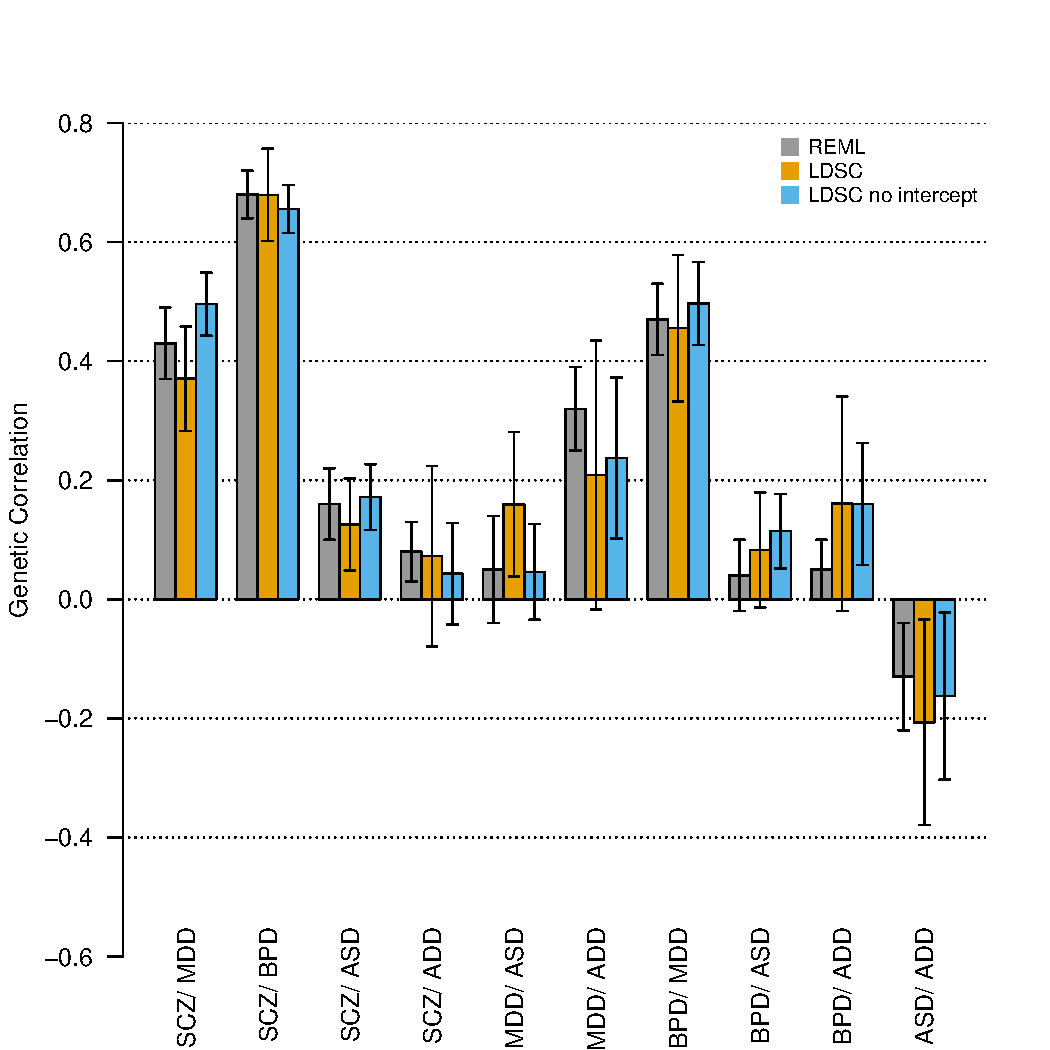
\includegraphics[scale=0.8]{figs/ldsc_vs_gcta.pdf}
         \label{Fig:Replication of PGC Cross Disorder Results}

\end{centering}

This plot compares LD Score regression estimates of genetic correlation using the summary statistics from \cite{cross2013identification} (which were generated from approximately the same data as \cite{pgccdg2013}) to 
estimates obtained from REML in \cite{pgccdg2013}.
The horizontal axis indicates pairs of phenotypes, and the vertical axis indicates genetic correlation.
Colors indicate different estimation procedures. Grey is REML,
Orange is HM3 LD Score with intercept; blue is HM3 LD Score without intercept, and green is partitioned 1kG LD Score
without intercept and with breakpoints at DAF=0.1, 0.3, 0.5, 0.7, 0.9 and recombination rate 0.05, 0.25, 1, 2 cM/Mb.
The estimates of genetic correlation between psychiatric phenotypes presented under the header 
``Application to a Large Set of Publicly Available Summary Statistics" use larger sample sizes, and so are more reliable;
this plot is intended primarily as a technical sanity check.
Abbreviations: 
ADD = Attention Deficit Hyperactivity Disorder (1947 trio cases, 1947 trio pseudocontrols, 840 cases, 688 controls);
ASD = Autism Spectrum Disorder (4788 trio cases, 4788 trio pseudocontrols, 161 cases, 526 controls);
BPD = Bipolar Disorder (6990 cases, 4820 controls);
MDD = Major Depressive Disorder (9227 cases, 7383 controls);
SCZ = Schizophrenia (9379 cases, 7736 controls).

\end{figure}

\subsubsection{Application to a Large Set of Publicly Available Summary Statistics}
We applied our method to \textbf{NUMBER} publicly available sets of GWAS summary statistics,
including   
schizophrenia \cite{schizophrenia2014biological}, 
major depression \cite{ripke2012mega}, 
bipolar disorder \cite{sklar2011large}, 
autism \cite{cross2013identification},
attention-deficit hyperactivity disorder \cite{neale2010meta},
anorexia \cite{boraska2014genome},
height \cite{allen2010hundreds}, 
body mass index \cite{speliotes2010association}, 
waist-hip ratio \cite{heid2010meta}, 
obesity \cite{berndt2013genome}, 
various insulin- and glucose- related traits
\cite{manning2012genome},
cigarettes per day,
age of onset of smoking,
ever vs never smokers,
former vs current smokers \cite{tobacco2010genome},
coronary artery disease \cite{schunkert2011large}, 
type-2 diabetes \cite{morris2012large}, 
rheumatoid arthritis \cite{stahl2010genome}, 
high-density lipoprotein,
low-density lipoprotein,
triglycerides,
total cholesterol \cite{teslovich2010biological},
ulcerative colitis \cite{jostins2012host},
Crohn's disease \cite{jostins2012host} and 
Alzhiemer's disease \cite{lambert2013meta}.
   
We estimated all pairwise genetic correlations between these phenotypes using the same two LD Scores from figure 
\ref{Fig:Replication of PGC Cross Disorder Results}.
Because the majority of these studies share some samples, we did not constrain any of the LD Score regression intercepts.
The genetic correlation estimates obtained using partitioned LD Score regression 
are displayed as a heatmap in Figure \ref{Fig:300 Gencors};
the genetic correlation estimates obtained with HM3 LD Scores are displayed as a heatmap in Supplementary Table \textbf{NNN},
and the full set of genetic correlation estimates are provided in tabular (\texttt{csv}) format in the Supplementary Data.
The differences between the genetic correlation estimates obtained from partitioned 1kG LD Scores and HM3 LD Scores were
not large \textbf{SUPPLEMENTARY FIGURE NNN}, 
indicating that -- at least for these phenotypes -- 
the extent to which genetic correlation depends on MAF or LD is not sufficient to introduce substantial bias.



The standard error of the genetic correlation estimate depends not only on sample size but also heritability.
As a rule of thumb, the higher the heritability $Z$-score ($\hat{h}^2/\mathrm{se}(\hat{h}^2)$), the lower the standard error for genetic correlation,
even for GC-corrected data.
This is a general feature of ratio estimators and is not specific to LD Score regression:
it is difficult to produce an accurate estimate of $1/x$ when the random variable $x$ is close to zero.

\begin{figure}[!ht]

\begin{centering}
\caption{Genetic Correlations Between 25 Published GWAS}
    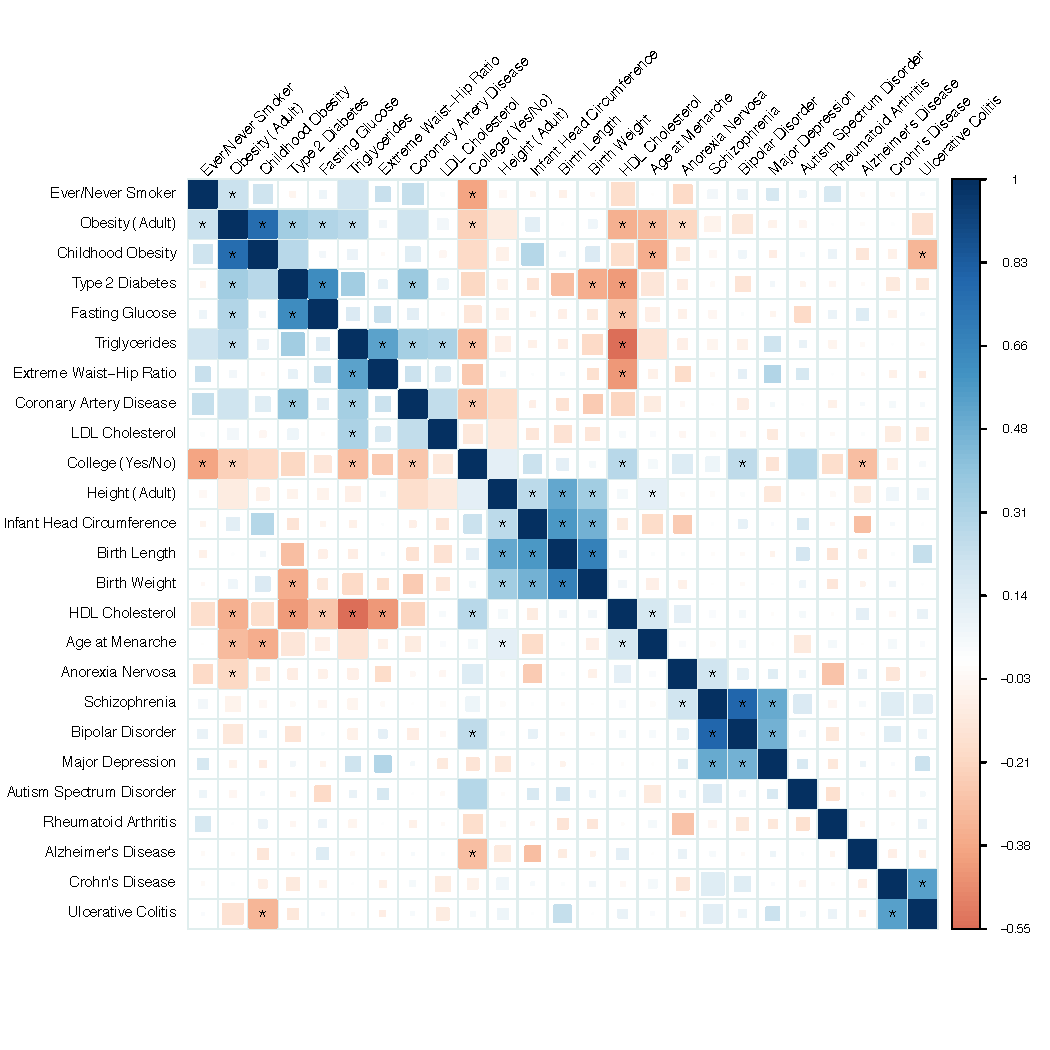
\includegraphics[scale=0.9]{figs/rg_heatmap.pdf}
         \label{Fig:300 Gencors}

Placeholder figure (HM3 LD Score). Caption goes here.
\end{centering}
\end{figure}
We find that phenotypes tend to cluster into categories defined by clinical practice and observational epidemiology;
for instance, we observe high genetic correlations between anthopometric traits, between psychiatric traits,  between 
metabolic traits and between autoimmune traits.
Reassuringly, most genetic correlations across pre-defined phenotypic categories were within not significantly different from
zero.
%%% FACTOR ANALYSIS?

Nevertheless, we observed some interesting examples of large genetic correlations that cut across phenotypic boundaries 
(Table \textbf{NNN}).
A few examples:
We estimate genetic correlations close to zero between Alzheimer's disease (AD) and all of the psychiatric traits.
Even though AD is classified as a psychiatric disorder in ICD-10, it appears to be genetically distinctive. 
Instead, AD clusters (weakly, but significantly) with anthopometric and metabolic traits.
We estimate genetic correlation close to zero between rheumatoid arthritis (RA) and schizophrenia, 
and between smoking traits and schizophrenia,
despite reduced risk of RA in patients with schizophrenia
and high rate of smoking in patients with schizophrenia

\textbf{COOL EXAMPLES?}

\subsection{Heritability}

The majority of the summary statistics that we analyzed were ``corrected'' via genomic control correction. 
This procedure yields downward bias in the LD Score regression estimates of heritability and genetic covariance 
\cite{buliksullivan2014} (though it does not affect genetic correlation). 
Thus, we can only present heritability estimates for the subset of GWAS that did not use GC correction.

We had information on sample MAF and imputation quality for these schizophrenia, CD and UC,
so we used all 1kG SNPs with sample MAF above 3\% and INFO above 0.9 for these LD Score regressions, 
since using a larger set of SNPs or the regression decreases the standard error.  
We estimated heritability using the same partitioned LD Scores as in figure \ref{Fig:300 Gencors},
both with and without constraining the LD Score regression intercept to equal one. 

Heritability estimates for UC, CD, SCZ and BPD are displayed in table \ref{Table:h2}.
\begin{table}[ht]
\centering
\caption{Heritability Estimates}
\label{Table:h2}
\begin{tabular}{rllll}
  \hline
\input{./table/h2}\label{Table:h2}
\end{tabular}

Liability scale heritability estimates for CD, UC, SCZ and BPD.
The first row contains estimates of $h^2_{5\myhyphen50\%}$ from LD Score regression with intercept constrained to one.
The second row contains estimates of $h^2_{5\myhyphen50\%}$ from LD Score regression with unconstrained intercept.
The LD Score regressions for CD, UC and SCZ used approximately 6 million well-imputed (INFO $>$ 0.9) 1kG SNPs. 
The LD Score regression for BPD used only HM3 SNPs.
All LD Score regressions in this table used a DAF $\times$ LD Score partitioned LD Score regression model with 35 bins. 
The estimates of $h^2_g$ for CD and UC are from \cite{chen2014estimation}; 
the estimates of $h^2_g$ for SCZ and BPD are from \cite{pgccdg2013}.
The prevalence row contains the population prevalences used for transformation to the liability scale. 
We note that estimates of liability scale heritability should be interpreted cautiously, since prevalence estimates
for many diseases are somewhat fuzzy quantities.
\end{table}


We also display estimates of $h^2_g$ from earlier publications, 
though we caution that $h^2_g$ and $h^2_{5\myhyphen50\%}$ are not the same quantity,
so any comparison between them is technically
apples-to-oranges (see the section $h^2_{5\myhyphen50\%}$ in the Methods).
The estimates of $h^2_g$ in table \ref{Table:h2} were obtained using REML on ascertained samples, 
and so are biased downwards \cite{golan2013narrowing}.
The heritability estimates with constrained intercept differed from the estimates with unconstrained intercept by less than one
standard error in all cases except for UC, where the difference was substantial. 
This could be explained either 
by a small amount of residual population stratification in the summary statistics (even after careful QC), 
reference/target LD mismatch or (most likely) model misspecification bias not fully accounted for by the partitioning. 


%%%%%%%%%%%%%%%%%%%%%%%%%%%%%%%%%%%%%%%%%%%%%%%%%%%%%%%%%%%%%%%
\section{Discussion}\label{Discussion}
%%%%%%%%%%%%%%%%%%%%%%%%%%%%%%%%%%%%%%%%%%%%%%%%%%%%%%%%%%%%%%%\

We have described a method for estimating common variant heritability and
genetic correlation that requires only GWAS summary statistics as input data.
Our method is immune to case/control ascertainment, sample overlap, shared population stratification \cite{buliksullivan2014}, 
and can be easily modified to be protected from bias from MAF- and LD-dependent genetic architectures. 
The computational demands of our method are mild: a few minutes on a standard laptop, irrespective of sample size.
Although LD Score regression does not use individual-level data,
the increase in standard error relative to methods that do use individual genotype and phenotype data is only moderate. 
In fact, LD Score regression without intercept is equivalent to HE regression in the non-partitioned case.

We note some limitations of LD Score regression. 
First, LD Score regression requires large sample sizes (at least several thousand) in order to give estimates with reasonable
standard error. 
For smaller sample sizes, REML is a more statistically efficient estimator of genetic correlation when its assumptions
are met (in particular, for non-ascertained studies) and individual genotypes are available.
In our opinion, figuring out how to obtain an efficient estimate of genetic correlation from a small and highly ascertained
sample (\emph{e.g.,} a study of a rare polygenic disease, 
where finding even a few thousand cases to genotype may be challenging) is an open question.

Second, LD Score regression assumes that all individuals in the GWAS were sampled from populations with similar LD Scores,
and that these LD Scores can be estimated from sequence data.
For multi-continental GWAS, the solution is to run LD Score regression on each continental subcohort separately, 
but nevertheless, LD Score regression can only be applied to samples from populations for which there exists a large 
sequenced reference panel. 
Currently, LD Score regression cannot be applied to samples from admixed populations.

Third, while genetic correlations are less confounded than overall phenotypic correlations from observational
epidemiology, genetic correlations cannot be interpreted as causal effects, even genetic correlations between intermediate 
phenotypes and disease.
For example, consider the strong positive genetic correlation between LDL and CAD in Figure \ref{Fig:300 Gencors}.
This genetic correlation could result from a causal effect, \emph{e.g.,} $\mathrm{LDL}\rightarrow\mathrm{CAD}$,
but could also result from non-causal shared genetic etiology 
\emph{e.g.,} $\mathrm{LDL}\leftarrow\mathrm{G}\rightarrow\mathrm{CAD}$, where $\mathrm{G}$ is some set of 
unknown genetic factors.
In this case, it is likely that LDL does cause CAD, because LDL-lowering drugs have been shown to decrease risk for CAD
in clinical trials; however, developing methods to distinguish between these models on the basis of genetic data alone is a 
particularly exciting direction for future research.

Finally, it is impossible to obtain any estimates of genetic correlation at all unless researchers are willing to share full sets of GWAS 
summary statistics! 
Since summary statistics contain such a large amount of information about genetic architecture and the relationships between 
phenotypes, it is surely the case that the benefits of data sharing outweigh the costs.
To facilitate data sharing, we have written a short guide describing the necessary information under 
the header ``Minimum Viable Summary Statistics'' in the Methods.


\newpage
%%%%%%%%%%%%%%%%%%%%%%%%%%%%%%%%%%%%%%%%%%%%%%%%%%%%%%%%%%%%%%%
\section{Online Methods}\label{Online Methods}
%%%%%%%%%%%%%%%%%%%%%%%%%%%%%%%%%%%%%%%%%%%%%%%%%%%%%%%%%%%%%%%

%%%%%%%%%%%%%%%%%%%%%%%%%%%%%%%%%%%%%%%%%%%%%%%%%%%%%%%%%%%%%%%
\subsection{Statistical Framework}
%%%%%%%%%%%%%%%%%%%%%%%%%%%%%%%%%%%%%%%%%%%%%%%%%%%%%%%%%%%%%%%

See the supplementary note for a thorough derivation of the models behind LD Score regression.


%%%%%%%%%%%%%%%%%%%%%%%%%%%%%%%%%%%%%%%%%%%%%%%%%%%%%%%%%%%%%%%
\subsection{$h^2_{5\myhyphen50\%}$}\label{h2550}
%%%%%%%%%%%%%%%%%%%%%%%%%%%%%%%%%%%%%%%%%%%%%%%%%%%%%%%%%%%%%%%

Let $S$ denote the set of all SNPs in 1000 Genomes (or whatever much larger sequenced reference panel future readers
are more familiar with); let $X_j$ denote the random variable whose value is the 0-1-2 coded genotype at SNP $j$, and let $y$
denote a phenotype. Let 
\begin{equation}
	\beta := \mathrm{argmax}_\alpha\left( \corr\left[y, \sum_{j\in S} X_j\alpha_j\right]^2 \right)
\end{equation}
(uniqueness of $\beta$ is guaranteed because this is a projection). 
Let $S'$ denote the set of SNPs with MAF$>5\%$. Then
\begin{equation}
	h^2_{5\myhyphen50\%} := \sum_{j\in S'} \beta_j^2.
\end{equation}
We choose 5\% as the lower bound, because we can estimate LD Scores for 5\% SNPs reasonably well from the $N=387$ 
samples in 1000 Genomes. With larger sample sizes in future sequenced reference panels, this lower bound can be pushed lower.

The main distinction between $h^2_{5\myhyphen50\%}$ and $h^2_g$ is that the effects of causal 4\% SNPs are not counted towards $h^2_{5\myhyphen50\%}$
This differs from the definition of the quantity $h^2_g$ estimated by REML, in that REML considers a set of SNPs
$g$, and then projects the phenotype onto those SNPs, without accounting for SNPs that are not in the set $g$. 
Thus if there is a 5\% SNP in set $g$ that is in high LD with a 4\% SNP that happens to be causal for the phenotype of interest
but is not in $g$, then the effect of the 4\% SNP is counted towards $h^2_g$ (or at least the component of the effect of 
the 4\% SNP that is tagged by the 5\% SNP that is in $g$).
There tends not to be very much LD between SNPs with different MAFs, 
so in the specific case of a MAF cutoff, this distinction likely makes only a small difference.

Technically, we should write $h^2_{5\myhyphen50\%,1kG}$ to indicate that we are only accounting for SNPs in 1000 Genomes,
but 1000 Genomes has sufficiently good power to observe 5\% and higher SNPs that we feel justified in omitting $1kG$
from the subscript for notational simplicity. 
It is perhaps more important to also note that we are only accounting for autosomal variation.
Most GWAS do not report summary statistics for SNPs on the sex chromosomes or in mitochondrial DNA.

Estimates of  $h^2_{5\myhyphen50\%}$ should generally be less than pedigree-based estimates of heritability
(modulo standard error), since pedigree estimators take into account all forms of genetic variation 
rare variants, microsatellites, indels, copy number variants, non-autosomal variation, etc).

The genetic covariance and genetic correlation quantitates that we estimate are direct bivariate analogues of 
$h^2_{5\myhyphen50\%}$. 
It is possible that the genetic covariance between two phenotype may be different among MAF$>5\%$ variants than
among rare variants; however, we could not detect such a phenomenon with GWAS data, since current GWAS only reliably
assay common variation.


%%%%%%%%%%%%%%%%%%%%%%%%%%%%%%%%%%%%%%%%%%%%%%%%%%%%%%%%%%%%%%%
\subsection{Estimation of LD Scores}
%%%%%%%%%%%%%%%%%%%%%%%%%%%%%%%%%%%%%%%%%%%%%%%%%%%%%%%%%%%%%%%

We estimated LD Scores from the European samples in the 1000 Genomes Project \cite{10002012integrated}
reference panel using the \texttt{--l2} flag in the \texttt{ldsc }software package by the authors (URLs) as in \cite{buliksullivan2014}.
We estimated per-allele LD Scores using the \texttt{--per-allele} flag in \texttt{ldsc}, and
we estimated MAF-binned LD Scores using the \texttt{--cts-bin} and \texttt{--cts-breaks} flags in \texttt{ldsc}.
Following \cite{buliksullivan2014}, we estimated LD Scores using a 1 centiMorgan (cM) window
(with the \texttt{ldsc} flag \texttt{--ld-wind-cm 1}).
Unlike \cite{buliksullivan2014}, we used a MAF cutoff of $1\%$ when estimating LD Scores,
in order to reduce the impact of LD measurement error on our regressions.
Since we only include variants with MAF $> 5\%$ in LD Score regressions for estimating genetic correlation,
and because there is very little LD between variants with MAF $> 5\%$ and variants with MAF $< 5\%$, 
this is unlikely to impact our results. 

For the analyses with HapMap 3 \cite{international2010integrating} LD Scores,
we took the sum of $r^2$'s over the same subset of HapMap 3 SNPs retained for LD Score regression in
\cite{buliksullivan2014}, (that is, HapMap 3 SNPs with MAF $> 1\%$, excluding centromeres and regions with long-range LD)
using the \texttt{--keep} flag in \texttt{ldsc}.


%%%%%%%%%%%%%%%%%%%%%%%%%%%%%%%%%%%%%%%%%%%%%%%%%%%%%%%%%%%%%%%
\subsection{Partitioned LD Score Regression}
%%%%%%%%%%%%%%%%%%%%%%%%%%%%%%%%%%%%%%%%%%%%%%%%%%%%%%%%%%%%%%%

In partitioned LD Score regression, we cut the set of SNPs in our reference panel into bins, for example,
we might use five MAF bins, corresponding to MAF 0-10\%, 10-20\%, ... , 40-50\% (as in supplementary table 4 of \cite{pgccdg2013}).  
We allow the variance explained per SNP to vary from bin to bin, but assume that variance explained per SNP is (roughly) 
equal within each bin. 
This amounts to approximating the unknown function that maps MAF to variance explained per SNP with a locally 
constant approximation. 
This presents a bias/variance tradeoff: if the mesh of our locally constant approximation is too coarse 
(\emph{e.g.,} if we were to use two MAF bins instead of five), 
our locally constant approximation would be poor, and this would result in bias. 
On the other hand, if we use too many bins, the standard error of our estimates will increase. 
However, we show in the simulations under the header ``Misspecified Models of Genetic Architecture" that
we can remove almost all MAF- and LD-bias under realistic parameter settings using only a few tens of bins, which 
increases the standard error only modestly.
MAF- and LD- partitioned LD Scores can be estimated using the \texttt{--cts-bin} and  \texttt{--cts-breaks} flags
from our \texttt{ldsc} software.


%%%%%%%%%%%%%%%%%%%%%%%%%%%%%%%%%%%%%%%%%%%%%%%%%%%%%%%%%%%%%%%
\subsection{Binning on in-Sample LD Score}
%%%%%%%%%%%%%%%%%%%%%%%%%%%%%%%%%%%%%%%%%%%%%%%%%%%%%%%%%%%%%%%

When estimating MAF- (or DAF-) and LD-partitioned LD Scores, we partition on LD Score and MAF estimated from the 
1000 Genomes Europeans.
At small sample sizes, this could present an overfitting problem.
For example, if we estimate LD Scores noisily, the SNPs assigned to the low-LD bin will be a mixture of SNPs that actually belong
in the low LD bin and SNPs whose LD Scores were underestimated, just by chance. 
This magnitude of this problem decreases as the sample size used for estimating LD Scores increases:
our estimator of LD Score is consistent,
so at very large sample sizes, the amount of sampling error in the LD Score estimates becomes very small, and the only SNPs
that will be misclassified are those SNPs whose LD Scores are very close to the boundary.

The quantify the extent to which this form of bias might be affecting our 1kG LD Scores, we performed a series of simulations. 
We simulated phenotypes following the infinitesimal model with \emph{i.i.d.} per-normalized genotype SNP effects using the same 
genotypes from section \ref{Simulations}.
We then estimated partitioned heritability and genetic correlation using an LD-partitioned 1kG LD Score with 5 bins.
If the overfitting problem described above were a real concern at the sample size of 1kG, 
we would expect to see either biased heritability and genetic covariance estimates or biased estimates of partitioned heritability. 
Results from these simulations are displayed in supplementary table \textbf{NNN}.
We do not observe appreciable bias in these simulations, so we conclude that binning on in-sample LD Score when estimating 
LD-partitioned LD Scores is acceptable at the sample size of 1kG.


%%%%%%%%%%%%%%%%%%%%%%%%%%%%%%%%%%%%%%%%%%%%%%%%%%%%%%%%%%%%%%%
\subsection{Genetic Covariance Regression Weights} 
%%%%%%%%%%%%%%%%%%%%%%%%%%%%%%%%%%%%%%%%%%%%%%%%%%%%%%%%%%%%%%%

For heritability estimation, we use the LD Score regression weights derived in the 
supplementary note from \cite{buliksullivan2014}. 
The optimal regression weights for genetic covariance estimation are 
\begin{equation}
\var[\bhat_j\chat_j \,|\, \ell_j ] = 
	\left( 
		\frac{\hsqo\ell_j}{M} 
		+ 
		\frac{1-\hsqo}{N_1} 
	\right) \left(  
		\frac{\hsqt\ell_j}{M} 
		+ 
		\frac{1-\hsqt}{N_2}
	\right) 
	+ 					
	2\left( 
		\frac{\gencov\ell_j}{M} 
		+ 
		\frac{\rho N_s}{N_1N_2} 
	\right);
\end{equation}
(Supplementary Note) however, this quantity depends on both heritabilities, 
the genetic covariance and the number of overlapping samples,
which are often not known a priori, so some approximation is required.
In order to obtain approximate regression weights, 
we use heritability estimates from the single-phenotype LD Score regressions, then
we assume that $N_s$ is close enough to zero that the term $\rho N_s/N_1N_2$ is negligible
(though this default can be adjusted using the {-}{-}overlap and {-}{-}rho flags in \texttt{ldsc}),
and estimate a rough genetic covariance (which we only use for the regression weights)
using the aggregate estimator 
$$\hat{\rho}_{g, agg} := \frac{1}{\lbar\sqrt{N_1N_2}}\sum_{j=1}^M z_{1,j}z_{2,j},$$
where $\lbar$ denotes the mean LD Score among SNPs included in the regression.
These regression weights are only an approximation to the optimal weights,
but this will not introduce bias into the regression;
it will only increase the standard error. 
The standard errors for LD Score regressions with summary statistics 
from GWAS with sample size below 10,000 are low enough to be interpretable,
so non-optimality of the regression weights does not seem to be a major hindrance.

Users of our \texttt{ldsc} software package should note that when attempting to compute the genetic 
correlation between a trait and itself using the same GWAS data twice, the result will generally be different from 
one unless the weights are set appropriately. 
With the default weights (which are set for zero sample overlap), \texttt{ldsc} is simply computing the ratio
between the slope of and LD Score regression with efficient weights and the slope of an LD Score regression
with inefficient regression weights, which is equal to one in expectation, but with noise.

%%%%%%%%%%%%%%%%%%%%%%%%%%%%%%%%%%%%%%%%%%%%%%%%%%%%%%%%%%%%%%%
%\subsection{LD Score Regression Intercept}
%%%%%%%%%%%%%%%%%%%%%%%%%%%%%%%%%%%%%%%%%%%%%%%%%%%%%%%%%%%%%%%

%As described in \cite{buliksullivan2014}, including an intercept in the LD Score regression protects against QC problems 
%(population stratification, cryptic relatedness) and sample overlap; however, these advantages come at the cost of a substantial
%increase in standard error. 
%This is unavoidable when dealing with summary statistics from large meta-analyses that do not
%share individual genotype data, since it is not otherwise possible to correct for sample overlap, and since 
%LD Score regression with constrained intercept can be badly biased when applied to summary statistics generated with GC
%correction, since GC correlation chances the expectation of the intercept \cite{buliksullivan2014}.
%However, if all individual genotypes are available for two studies for which we want to compute genetic correlation,
%the most efficient approach is the following:
%\begin{enumerate}
%\item If the phenotype is a quantitative trait or a non-ascertained binary trait, use REML. For ascertained binary traits,
%REML is biased, and LD Score regression with constrained intercept is the most efficient estimator.
%\item Perform careful QC (\emph{e.g.,} removing ancestry outliers, PCA, etc) \emph{before} computing summary statistics.
%\item Estimate heritability with the LD Score regression intercept constrained to one. It may be useful to run LD Score regression with intercept as a model check: intercepts much larger than one after population stratification has been excluded can indicate model misspecification bias. 
%\item Estimate genetic covariance with the LD Score regression intercept constrained to $\rho N_s/N_1N_2$, where $\rho$ denotes the phenotypic correlation among individuals who appear in both studies (this expression equals zero if there is no sample overlap).
%\end{enumerate}

%The choice of whether to use in-sample LD from imputed genotype data vs. out-of-sample LD from a sequenced reference panel implicitly changes the model, as discussed in section \ref{PGCCDG}; however, with densely imputed genotyped data
%(for instance, if using 1kG as the imputation reference), the difference will be small, especially for genetic correlation.

%%%%%%%%%%%%%%%%%%%%%%%%%%%%%%%%%%%%%%%%%%%%%%%%%%%%%%%%%%%%%%%
\subsection{Weighted Block Jackknife Genetic Correlation}
%%%%%%%%%%%%%%%%%%%%%%%%%%%%%%%%%%%%%%%%%%%%%%%%%%%%%%%%%%%%%%%

This section describes the implementation of the \texttt{--sumstats-gencor} flag in \texttt{ldsc}.

Genetic correlation is defined as a ratio of quantities: 
\begin{equation*}
	r_g := \frac{\gencov}{\sqrt{\hsqo\hsqt}}.
\end{equation*}
Instead of the naive estimator of this ratio, 
\begin{equation*}
	\rhat_{g} := \frac{\hat{\rho}_g }{ \sqrt{\hat{h}^2_1\hat{h}^2_2}},
\end{equation*}
we use the weighted block jackknife estimator \cite{busing1999delete} of the ratio, 
with the jackknife taken over blocks of adjacent SNPs
\begin{equation}
    \hat{r}_{g,jack} := 
    n_b\hat{r}_{g} -
     \sum_{i=1}^{n_b}
     	\left(1-\frac{m_i}{M_g}\right)\hat{r}_{g,i}
\end{equation}
where $n_b$ is the number of blocks, and $\hat{r}_{g,i}$ is
the naive estimate of genetic correlation obtained by deleting the $i^{th}$ block of SNPs, 
$m_i$ is the number of SNPs in block $i$, and $M_g$ is the number of SNPs included in the regression.
The weighted block jackknife ratio estimator is less biased than the naive estimate (though this is not so important at our sample sizes), 
and comes with a convenient nonparametric variance estimator \cite{busing1999delete},
\begin{equation}
    \widehat{\mathrm{Var}}\left[\hat{r}_{g,jack}\right] 
:= 
    \frac{1}{n_b} \sum_{i=1}^{n_b}
    	\frac{1}{h_i - 1}
	\left(
		(h_i-n_b)\hat{r}_g - (h_i-1)\hat{r}_{g,i} + \sum_{j=1}^{n_b} \left(1-\frac{m_i}{M_g}\hat{r}_{g,j}\right),
		\right)
\end{equation}
where $h_i := M_g / m_i$.
Weighted block jackknife standard errors (over blocks of adjacent SNPs) 
are robust to the  correlated error structure of GWAS $\chi^2$-statistics, 
so long as the block size exceeds the typical range of LD. 
See references \cite{buliksullivan2014, finucane2014partitioning, moorjani2011history} 
for examples of papers in the statistical and population genetics literature that use this technique. 
We checked the reliability of our standard errors via simulations with real genotypes
(Supplementary Table \ref{supp-se_sim}),
and found that the \texttt{ldsc} default setting  of 2000 blocks genome-wide
(which can be adjusted with the \texttt{--num-blocks} flag) gives standard error estimates
that agree well with the empirical standard deviation across simulation replicates.

In another set of simulations with much lower power (not shown), we observed that the LD Score regression
genetic correlation estimates became unstable when either sample size or heritability was so low that at least one 
of the two heritability estimates was not significantly different from zero. 
This is a general difficult with attempting to estimate a ratio where the denominator is close to zero, and is not 
specific to LD Score regression. 
As a rule of thumb, 
we recommend discarding (or at least being very cautious with) 
any genetic correlation estimates where either of the following conditions is met:
\begin{enumerate}
	\item Either of the heritability estimates is less than 2 SE's from zero, or
	\item The block jackknife SE for the genetic correlation estimate is greater than 0.2.
\end{enumerate}


%%%%%%%%%%%%%%%%%%%%%%%%%%%%%%%%%%%%%%%%%%%%%%%%%%%%%%%%%%%%%%%
\subsection{GWAS Data}
%%%%%%%%%%%%%%%%%%%%%%%%%%%%%%%%%%%%%%%%%%%%%%%%%%%%%%%%%%%%%%%

\subsubsection{Minimum Viable Summary Statistics}

The minimum summary data required for estimating genetic correlation with LD Score regression are the following:
\begin{enumerate}
	\item Genome-wide summary statistics from cohorts with similar ancestry
	\item The summary statistics must be \emph{signed} (allele and direction of effect)
	\item The summary statistics should \emph{never} be ``corrected'' via genomic control (GC) correction. Using GC'ed
		summary statistics will result in downward bias in the LD Score regression estimates of heritability and
		genetic covariance, and deflated LD Score regression intercepts, though the genetic correlation estimates will be fine.
	\item The summary statistics must not be meta-analyzed with targeted genotyping at significant loci 
		(\emph{e.g.,} specialty genotyping arrays like immunochip, exome chip, psychchip, metabochip, or replication cohorts). 		LD Score regression is currently not applicable to data generated using custom genotyping arrays 
		Although REML has been applied to such datasets, we suspect these results may have been biased due to the 
		non-random selection of genotyped SNPs. 

\end{enumerate}
The next details are nice to have, but are only used for filtering SNPs:
\begin{enumerate}
	\item A measure of imputation quality (\emph{e.g.,} INFO) for each SNP
	\item Sample size at each SNP (for binary traits, number of cases and number of controls)
	\item Sample MAF
\end{enumerate}
If these data are not available, 
we recommend retaining only HapMap 3 SNPs with reference panel MAF above 5\% for the LD Score regression as a workaround
(note: for \emph{regression}, not for estimation of the LD Scores), 
since HapMap3 SNPs seem to be well-imputed in most studies.
For newer studies with dense imputation, restricting to HapMap 3 SNPs is an inefficient use of data. 
Using a larger set of SNPs for the regression will lower the standard error (\emph{e.g.,} using all common 1kG
SNPs instead of all common HM3 SNPs for the regression reduces the standard error by about 10\% in simulations).

Since INFO scores are only used for filtering, researchers unwilling to share INFO scores should consider sharing a binary
variable indicating the SNPs for which the INFO score was above 0.9.

\subsubsection{Huge Effect Loci}

Though the derivation of LD Score regression makes no distributional assumptions about effect sizes, 
the LD Score regression standard error can become very large if effect sizes are drawn from a highly kurtotic distribution,
\emph{i.e.,} if there are huge-effect loci. 
The \texttt{ldsc} default is to remove a window around SNPs with $\chi^2 > 0.01N$
(this can be disabled with the \texttt{--no-filter-chisq} flag).


\subsubsection{IGAP}

IGAP (which provided the summary statistics for Alzheimer's disease) requests that we include the following text in our methods section:
\begin{quotation}
    International Genomics of Alzheimer's Project (IGAP) is a large two-stage study based upon genome-wide association studies (GWAS) on individuals of European ancestry. 
    In stage 1, IGAP used genotyped and imputed data on 7,055,881 single nucleotide polymorphisms (SNPs) to meta-analyze four previously-published GWAS datasets consisting of 17,008 Alzheimer's disease cases and 37,154 controls 
    (The European Alzheimer's disease Initiative, EADI; the Alzheimer Disease Genetics Consortium, ADGC; The Cohorts for Heart and Aging Research in Genomic Epidemiology consortium, CHARGE; The Genetic and Environmental Risk in AD consortium, GERAD). 
    In stage 2, 11,632 SNPs were genotyped and tested for association in an independent set of 8,572 Alzheimer's disease cases and 11,312 controls. 
    Finally, a meta-analysis was performed combining results from stages 1 and 2.
\end{quotation}
We only used stage 1 data for LD Score regression.

\newpage
%%%%%%%%%%%%%%%%%%%%%%%%%%%%%%%%%%%%%%%%%%%%%%%%%%%%%%%%%%%%%%%
%\input{./tex/main/legends}
%%%%%%%%%%%%%%%%%%%%%%%%%%%%%%%%%%%%%%%%%%%%%%%%%%%%%%%%%%%%%%%


%%%%%%%%%%%%%%%%%%%%%%%%%%%%%%%%%%%%%%%%%%%%%%%%%%%%%%%%%%%%%%%
\section{URLs}\label{URLs}
%%%%%%%%%%%%%%%%%%%%%%%%%%%%%%%%%%%%%%%%%%%%%%%%%%%%%%%%%%%%%%%

\begin{enumerate}
	\item \texttt{ldsc} software:\\ 
		\texttt{github.com/bulik/ldsc}
		
	\item LD block genotype simulation code:\\
		\texttt{github.com/bulik/ldsc-sim}
		
	\item This paper:\\
		\texttt{github.com/bulik/gencor\_tex}
		
	\item PGC (psychiatric) summary statistics:\\ 
		\texttt{www.med.unc.edu/pgc/downloads}
		
	\item GIANT (anthopometric) summary statistics: \\
		\texttt{www.broadinstitute.org/collaboration/giant/index.php/GIANT\_consortium\_data\_files}
		
	\item MAGIC (insulin, glucose) summary statistics: \\
		\texttt{www.magicinvestigators.org/downloads/}
		
	\item CARDIoGRAM (coronary artery disease) summary statistics:\\	
		\texttt{www.cardiogramplusc4d.org}
	
	\item DIAGRAM (T2D) summary statistics:\\
		\texttt{www.diagram-consortium.org}
		
	\item Rheumatoid Arthritis summary statistics:\\
		\texttt{www.broadinstitute.org/ftp/pub/rheumatoid\_arthritis/Stahl\_etal\_2010NG/}
	
	\item IGAP (Alzheimers) summary statistics:\\
		\texttt{www.pasteur-lille.fr/en/recherche/u744/igap/igap\_download.php}

	\item IIBDGC (inflammatory bowel disease) summay statistics:\\
		\texttt{www.ibdgenetics.org/downloads.html}\\
		We used a newer version of these data with 1000 Genomes imputation.

	\item Plasma Lipid summary statistics:\\
		\texttt{www.broadinstitute.org/mpg/pubs/lipids2010/}
	
	\item Beans:\\
		\texttt{www.barismo.com}\\
		\texttt{www.bluebottlecoffee.com}
\end{enumerate}

\newpage
%%%%%%%%%%%%%%%%%%%%%%%%%%%%%%%%%%%%%%%%%%%%%%%%%%%%%%%%%%%%%%%
\section{Acknowledgements}\label{Acknowledgements}
%%%%%%%%%%%%%%%%%%%%%%%%%%%%%%%%%%%%%%%%%%%%%%%%%%%%%%%%%%%%%%%

We would like to thank P. Sullivan and S. Caldwell for helpful discussion. This work was supported by NIH grants R01 HG006399 (ALP), R03 CA173785 (HKF) and by the Fannie and John Hertz Foundation (HKF). The coffee that Brendan drank while writing this paper was roasted by Barismo in Arlington, MA and Blue Bottle Coffee in Oakland, CA. 

Data on glycaemic traits have been contributed by MAGIC investigators and have been downloaded from www.magicinvestigators.org.

Data on coronary artery disease / myocardial infarction have been contributed by CARDIoGRAMplusC4D investigators and have been downloaded from 
www.CARDIOGRAMPLUSC4D.ORG

We thank the International Genomics of Alzheimer's Project (IGAP) for providing summary results data for these analyses. The investigators within IGAP contributed to the design and implementation of IGAP and/or provided data but did not participate in analysis or writing of this report. IGAP was made possible by the generous participation of the control subjects, the patients, and their families. The i-Select chips was funded by the French National Foundation on Alzheimer's disease and related disorders. EADI was supported by the LABEX (laboratory of excellence program investment for the future) DISTALZ grant, Inserm, Institut Pasteur de Lille, Universit� de Lille 2 and the Lille University Hospital. GERAD was supported by the Medical Research Council (Grant 503480), Alzheimer's Research UK (Grant 503176), the Wellcome Trust (Grant 082604/2/07/Z) and German Federal Ministry of Education and Research (BMBF): Competence Network Dementia (CND) grant 01GI0102, 01GI0711, 01GI0420. CHARGE was partly supported by the NIH/NIA grant R01 AG033193 and the NIA AG081220 and AGES contract N01-AG-12100, the NHLBI grant R01 HL105756, the Icelandic Heart Association, and the Erasmus Medical Center and Erasmus University. ADGC was supported by the NIH/NIA grants: U01 AG032984, U24 AG021886, U01 AG016976, and the Alzheimer's Association grant ADGC-10-196728.


%%%%%%%%%%%%%%%%%%%%%%%%%%%%%%%%%%%%%%%%%%%%%%%%%%%%%%%%%%%%%%%
\section{Author Contributions}\label{author_contribs}
%%%%%%%%%%%%%%%%%%%%%%%%%%%%%%%%%%%%%%%%%%%%%%%%%%%%%%%%%%%%%%%

The caffeine molecule is responsible for everything that is good about this manuscript.
BBS and HKF are probably responsible for the other bits.
All authors revised and approved the final manuscript.


%%%%%%%%%%%%%%%%%%%%%%%%%%%%%%%%%%%%%%%%%%%%%%%%%%%%%%%%%%%%%%%
\section{Competing Financial Interests}
%%%%%%%%%%%%%%%%%%%%%%%%%%%%%%%%%%%%%%%%%%%%%%%%%%%%%%%%%%%%%%%

Unfortunately, we have no financial conflicts of interest to declare.

\newpage
\bibliographystyle{plain}
\bibliography{gencor}

\end{document}
